\documentclass[twocolumn, 12pt]{article}    % two-column because cheat sheets fit like that
\usepackage{preamble}
\newcommand\coursename{Intro to Robotics}

\begin{document}
\RaggedRight
\footnotesize % small because, it's a cheat sheet after all, why not cram it

\noindent
\underline{Coordinate Transforms} \(T\)\\
\textbf{Left-to-right} evaluation about the \textbf{current frame}\\

\noindent
\underline{Operators} \(D\)\\
\textbf{Right-to-left} evaluation about the \textbf{fixed frame}\\

\begin{equation*} 
    \text{let} \hspace{10pt}
    \begin{bmatrix}
        \prescript{1}{}{\Vec{q}}_1 \\ 1
    \end{bmatrix} = D_1 \begin{bmatrix}
        \prescript{1}{}{\Vec{p}}_1 \\1
    \end{bmatrix}, \hspace{10pt} \text{and we want} \hspace{10pt}\begin{bmatrix}
        \prescript{0}{}{\Vec{q}}_2 \\ 1
    \end{bmatrix} = D_0 \begin{bmatrix}
        \prescript{0}{}{\Vec{p}}_2 \\ 1
    \end{bmatrix} 
\end{equation*}
\begin{equation*}
    \text{then:}\hspace{10pt}
     \begin{bmatrix}
        \prescript{0}{}{\Vec{q}}_2 \\ 1
    \end{bmatrix} = \underbrace{\prescript{0}{}{T}_1 D_1 \prescript{0}{}{T}_1^{-1}}_{\text{tensor transform}} \begin{bmatrix}
        \prescript{0}{}{\Vec{p}}_2 \\ 1
    \end{bmatrix} = D_0\begin{bmatrix}
        \prescript{0}{}{\Vec{p}}_2 \\ 1
    \end{bmatrix} 
\end{equation*}



\noindent\underline{Forward Kinematics}
\begin{figure}[h!]
    \centering
    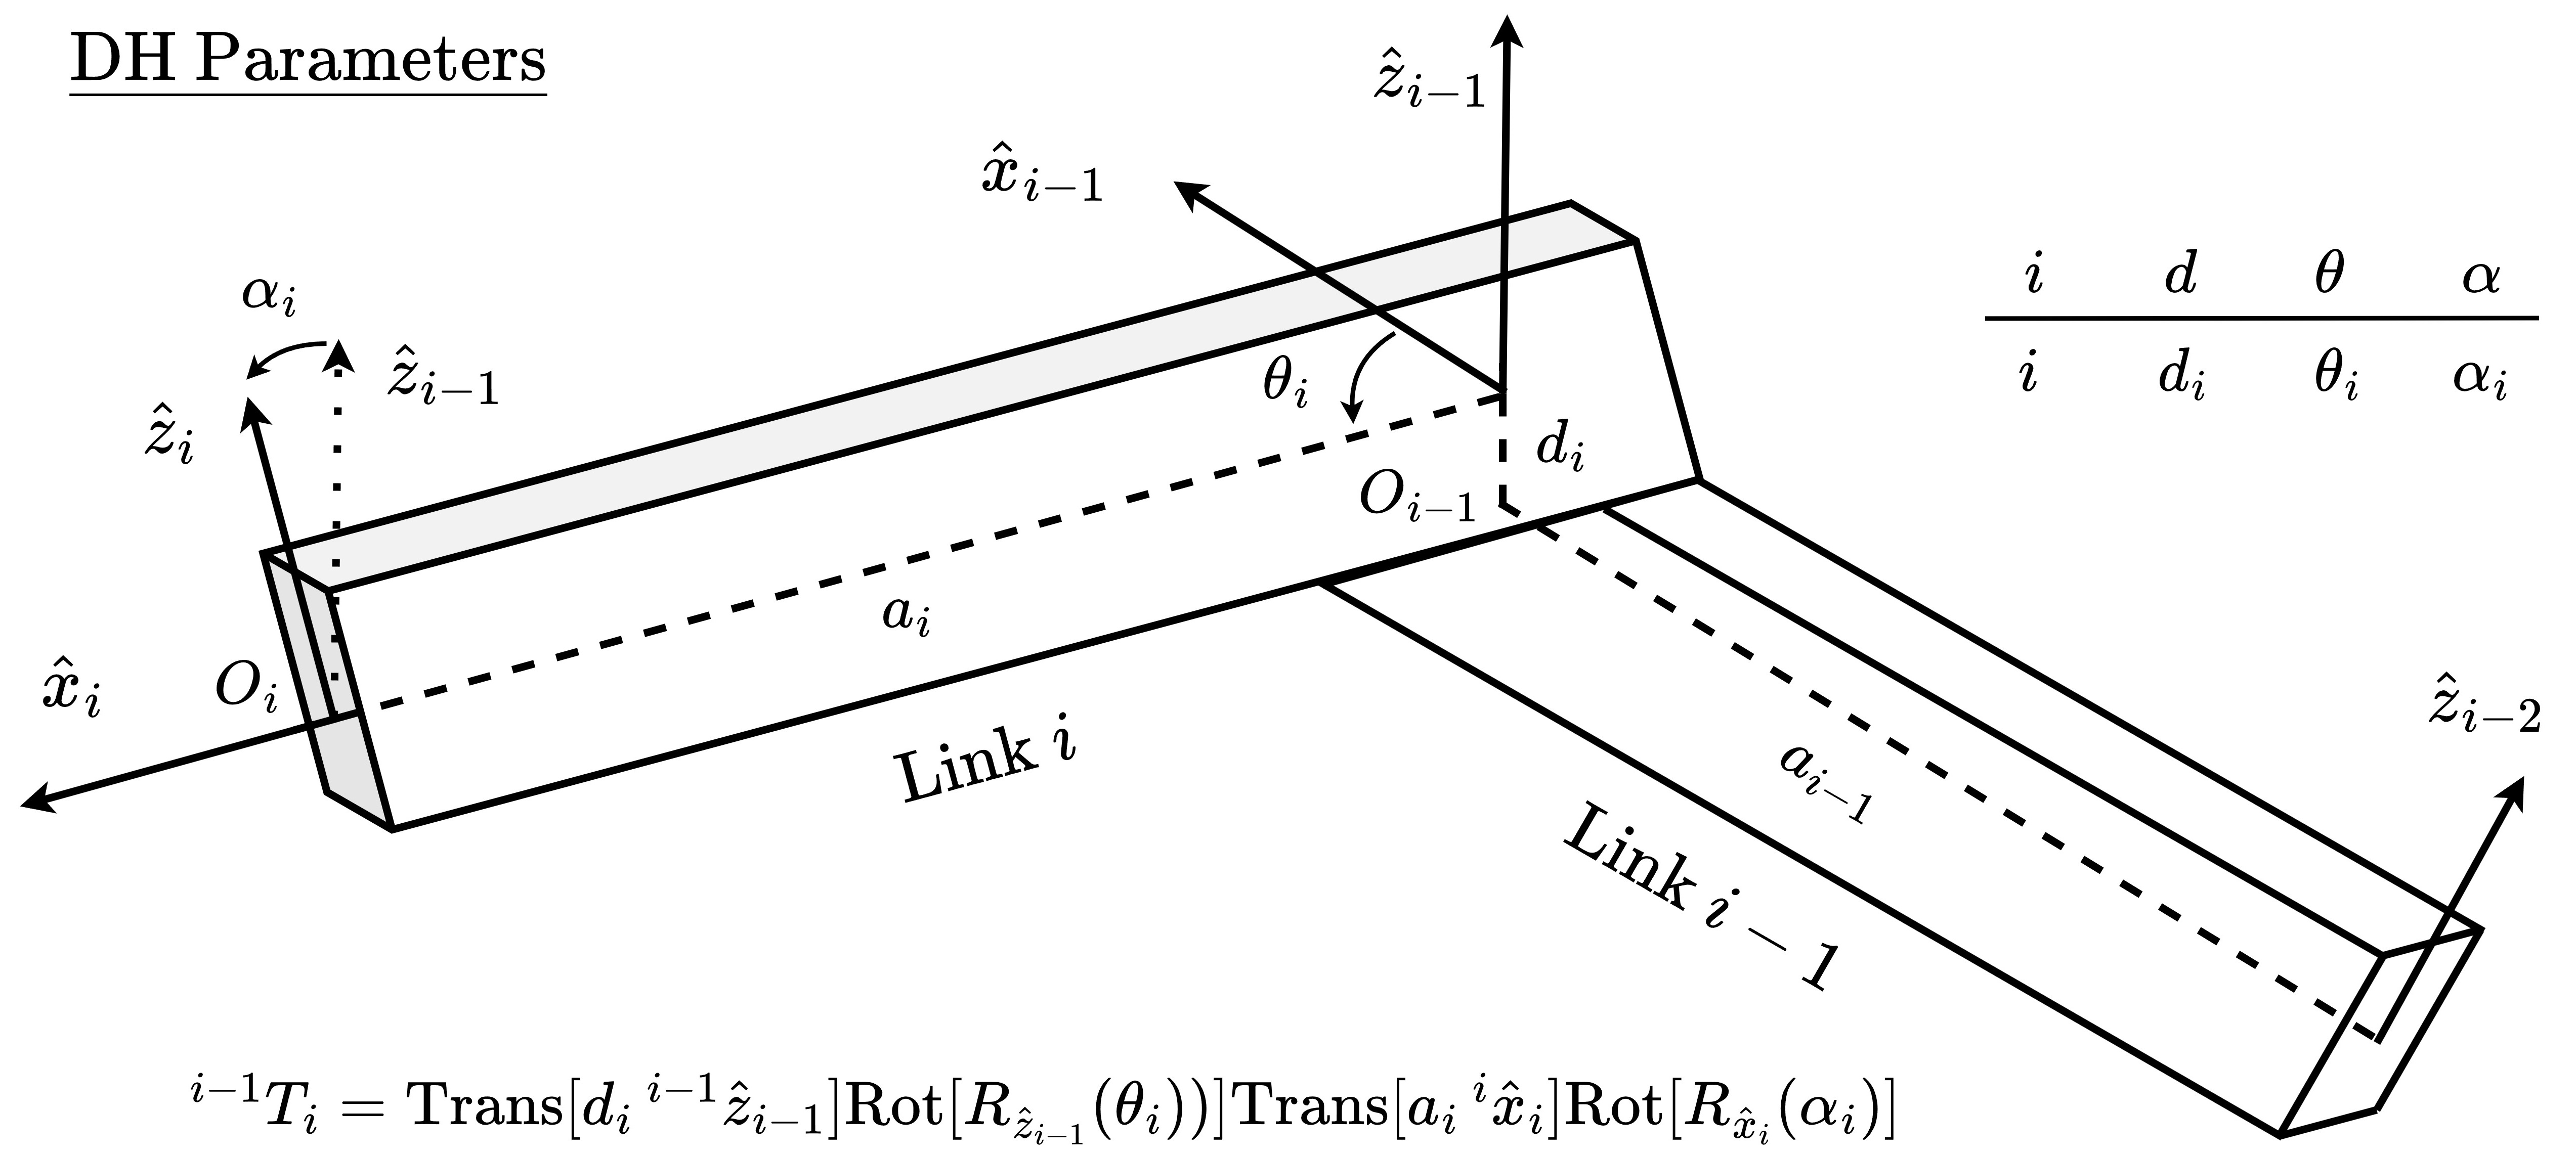
\includegraphics[width = 0.5\textwidth]{figures/DHParameters.jpg}
\end{figure}
\begin{itemize}
    \item Coordinate transform (L\(\to\)R about current frame)
    \item If \(\hat{z}_{i-1} \perp \hat{z}_i\), pick \(\hat{x}_i = \pm \hat{z}_{i-1} \times \hat{z}_i\)
    \item If \(\hat{z}_{i-1} \parallel \hat{z}_i\), pick \(\hat{x}_i\) to intersect \(O_{i-1}\) for kinem. calib.
    \item \(\prescript{-1}{}{T}_{\text{tool}} = \prescript{-1}{}{T}_0 \prescript{0}{}{T}_1 \dots \prescript{n-1}{}{T}_n \prescript{n}{}{T}_{\text{tool}}\)
    \item Don't care solution keeps last row of DH zeroes except the joint variable
\end{itemize}

\noindent\underline{Inverse Kinematics}\\
Find joint parameters \(\theta_i^*\) or \(d_i^*\) \(\forall i\), given \(\prescript{0}{}{\vec{d}}_{0n}\) and \(\prescript{0}{}{R}_{0n}\) 
\begin{equation*}
    \prescript{0}{}{\vec{d}_{0n}} = \begin{bmatrix}
        \prescript{0}{}{d}_{0n1} \\ \prescript{0}{}{d}_{0n2} \\ \prescript{0}{}{d}_{0n3}
    \end{bmatrix} \triangleq \begin{bmatrix}
        x \\ y \\ z
    \end{bmatrix} \hspace{30pt} \prescript{0}{}{R}_{0n} \triangleq \{r_{ij}\}
\end{equation*}
\begin{equation*}
    \theta = 2 \text{atan}\left( \pm \sqrt{\frac{1- \cos(\theta)}{1+ \cos(\theta)}}\right) \hspace{8pt} \text{ half angle tan formula for cos}
\end{equation*}
\begin{equation*}
    \prescript{i-1}{}{R}_i = R_{\hat{z}_{}-1}(\theta_i) R_{\hat{x}_i} (\alpha_i) \hspace{20pt} \prescript{i-1}{}{\vec{d}}_{i-1,i} = d_i \prescript{i-1}{}{\hat{z}}_{i-1} + a_i \prescript{i-1}{}{\hat{x}}_i
\end{equation*}
\begin{equation*}
    \prescript{0}{}{R}_n = \prescript{0}{}{R}_1 \dots \prescript{n-1}{}{R}_n \hspace{30pt} \prescript{0}{}{T}_n = \prescript{-1}{}{T}_0^{-1} \prescript{-1}{}{T}_{\text{tool}} \prescript{n}{}{T}_{\text{tool}}^{-1}
\end{equation*}
\begin{equation*}
    \prescript{0}{}{\Vec{d}}_{0n} = \sum_{k=1}^n d_k \prescript{0}{}{R}_{k-1} \prescript{k-1}{}{\hat{z}}_{k-1} + a_k \prescript{0}{}{R}_k \prescript{k}{}{\hat{x}}_k
\end{equation*}

\vspace{-7.5pt}
\noindent Pythagorean
\begin{itemize}
    \item If a convenient triangle can be drawn, use a Pythagorean method to solve for joint angles
    \vspace{-10pt} 
    \begin{equation*}
        c^2 = a^2 + b^2 -2ab\cos(C) \hspace{30pt} \begin{matrix}
            \text{w/ sides } a,\, b,\, c \text{ opposite} \\
            \text{to angles } A,\, B,\, C
        \end{matrix}
    \end{equation*}
\end{itemize}

Shadow Box/Line
\begin{figure}[h!]
    \centering
    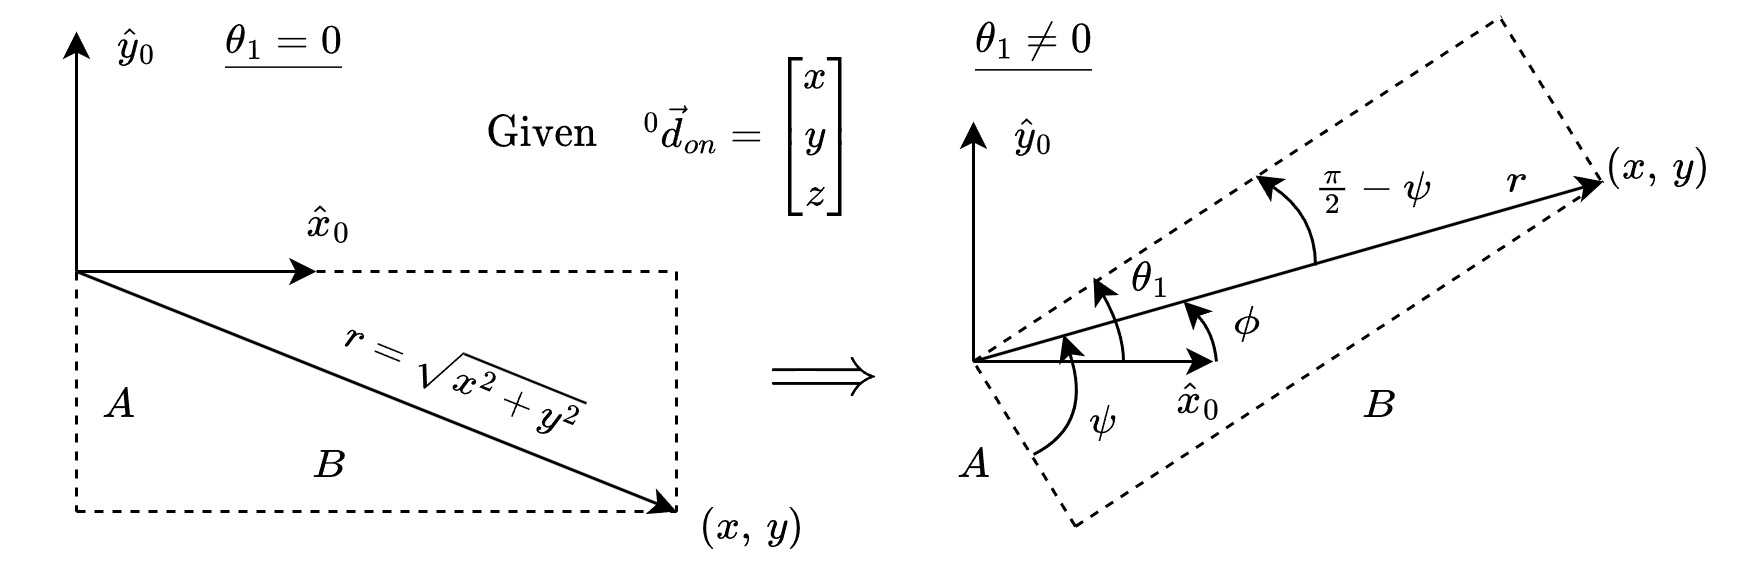
\includegraphics[width = 0.5 \textwidth]{figures/ShadowBox.jpg}
\end{figure}
\begin{enumerate}
    \item Find \(A,\, B\) by projecting onto a plane (usually \(\hat{x}_0 - \hat{y}_0)\)
    \item Introduce \(\phi\) and \(\psi\) such that \(\theta_1 = \phi + (\pi/2 -\psi)\)
    \item Solve for \(\phi = \text{atan2}(y,\, x)\) with \textbf{1 solution}
    \item Solve for \(\cos(\psi) =A/r\) or \(\sin(\psi) = \cos(\pi/2 + \psi) = B/r\) using the half angle tangent formula, based on what is known within \(A\) and \(B\), resulting in \textbf{2 solutions}
    \item Plug into \(\theta_1 = \phi + (\pi/2 -\psi)\), resulting in \textbf{2 solutions} because of \(\psi\)
\end{enumerate}

\noindent Projection/Influence Table 
\begin{itemize}
    \item Consider the spatial effect of perturbing each joint individually. If only a dimension (\(x,\, y,\, z\)) is affected by only one joint, project \(\prescript{0}{}{\vec{d}}_{0n}\) with that dimension, and find that joint variable
\end{itemize}


\noindent\underline{Euler Angles}
\begin{equation*}
    R_{ABC} = R_A(\phi) R_B(\theta)R_C(\psi) = \{r_{ij}\} \hspace{20pt} A,\, B,\, C \in \{\hat{x},\, \hat{y},\, \hat{z}\}
\end{equation*}
\begin{enumerate}
    \setcounter{enumi}{-1} 
    \item Write out each rotation matrix, and simplify to total rotation matrix 
    \item Find first angle by taking the ratio of two \(r_{ij}\) components s.t. they simplify to tan(\(\angle_1\)), and apply half angle tan to find \textbf{2 solutions} for \(\angle_1\)
    \item Find the \(r_{ij}\) that only includes one trig(\(\angle_2\)). Take two other \(r_{ij}\) and multiply by \(\sin/\cos\) to result in the complementary trig(\(\angle_2\)), then use atan2(\(\sin(\angle_2),\, \cos(\angle_2)\)) to find \textbf{1 solution} for \(\angle_2\) \label{euler step}
    \begin{equation*}
        \cos(\angle) r_{ij} + \sin(\angle)r_{ij} \text{ s.t. } = [\cos^2(\angle) + \sin^2(\angle)]\text{trig}(\angle_2)
    \end{equation*}
    \item Similar to step \ref{euler step}, perform the addition cancellation twice (using four \(r_{ij}\)) to achieve estimates for sin(\(\angle_3\)) and cos(\(\angle_3\)), then atan2(\(\sin(\angle_3),\, \cos(\angle_3)\)) to find \textbf{1 solution} for \(\angle_3\)
\end{enumerate}
If \(\sin(\theta)=0\), the rotation matrix is degenerate and becomes \(R_{ABC} = R_{AC}=R_A(\phi)R_C(\psi)\). If \(A=C\), it becomes \(R_A(\phi+\psi)\), where \(\phi\) and \(\psi\) cannot be uniquely solved. Convention is \(\phi=0\), and solve for \(\theta,\, \psi\).


\noindent\underline{Inverse Kinematic Velocities}\\
Solve for joint (positions, velocities, accelerations) in that order, given \(\prescript{0}{}{\dot{\vec{d}}}_{0n}\) or \(\prescript{0}{}{\vec{\omega}}_{0n}\) from trajectory planner\\
\vspace{10pt} 
''The time derivative of a fixed length vector is the angular velocity of the body w/ which it is fixed, crossed w/ the fixed length vector''
\begin{align*}
    \prescript{i-1}{}{\dot{R}}_i &= \dot{\theta}_i S(\prescript{i-1}{}{\hat{z}}_{i-1}) R_{\hat{z}}(\theta_i) \\
    &= S(\dot{\theta}_i \prescript{i-1}{}{\hat{z}}_{i-1}) R_{\hat{z}} (\theta_i) = \prescript{i-1}{}{\vec{\omega}_i} \times R_{\hat{z}}(\theta_i)
\end{align*}
\vspace{-20pt}
\begin{align*}
    \begin{matrix}
        \text{recursive} \\ \text{rotary}
    \end{matrix} \hspace{10pt}&
    \begin{cases}
        \prescript{0}{}{\dot{\vec{d}}}_{i-1, i} &= \prescript{0}{}{\vec{\omega}_{0i}} \times \prescript{0}{}{\vec{d}}_{i-1,i}\\
        \prescript{0}{}{\vec{\omega}}_{oi} &= \prescript{0}{}{\vec{\omega}}_{0,i-1} + \dot{\theta}_i \prescript{0}{}{\hat{z}}_{i-1} 
    \end{cases}\\
    \begin{matrix}
        \text{recursive} \\ \text{prismatic}
    \end{matrix}\hspace{10pt}&
    \begin{cases}
        \prescript{0}{}{\dot{\vec{d}}}_{i-1, i} &= \dot{d}_i^* \prescript{0}{}{\hat{z}}_{i-1} + \prescript{0}{}{\vec{\omega}_{0i}} \times \prescript{0}{}{\vec{d}}_{i-1,i} \\
        \prescript{0}{}{\vec{\omega}}_{oi} &= \prescript{0}{}{\vec{\omega}}_{0,i-1} + 0
    \end{cases}
\end{align*}
\vspace{-20pt} 
\begin{align*}
    \text{\rotatebox{90}{\hspace{-10pt}rotary}}&
    \begin{bmatrix}
        \prescript{0}{}{\dot{\vec{d}}}_{0n} \\ \prescript{0}{}{\vec{\omega}}_{0n} 
    \end{bmatrix} = J_v \dot{\vec{\theta}}=\begin{bmatrix}
        \prescript{0}{}{\hat{z}}_0 \cdot \prescript{0}{}{\vec{d}}_{0n} & \dots & \prescript{0}{}{\hat{z}}_{n-1} \cdot \prescript{0}{}{\vec{d}}_{n-1,n}\\
        \prescript{0}{}{\hat{z}}_0 & \dots & \prescript{0}{}{\hat{z}}_{n-1}
    \end{bmatrix} \begin{bmatrix}
        \dot{\theta}_1 \\ \vdots \\ \dot{\theta}_n
    \end{bmatrix}\\
    \text{\rotatebox{90}{\hspace{-17.5pt}prismatic}} &
    \begin{bmatrix}
        \prescript{0}{}{\dot{\vec{d}}}_{0n} \\ \prescript{0}{}{\vec{\omega}}_{0n} 
    \end{bmatrix} = J_v \dot{\vec{d}}= \begin{bmatrix}
        \prescript{0}{}{\hat{z}}_0  & \dots & \prescript{0}{}{\hat{z}}_{n-1} \\
        0 & \dots & 0
    \end{bmatrix} \begin{bmatrix}
        \dot{d}_1 \\ \vdots \\ \dot{d}_n
    \end{bmatrix} \hspace{22pt} \begin{matrix}
        \text{interweave}\\ \text{accordingly}
    \end{matrix}
\end{align*}
\vspace{-20pt}
\begin{enumerate}
    \item Write out \(\prescript{0}{}{\dot{\vec{d}}}_{0n}\) or \(\prescript{0}{}{\vec{\omega}}_{0n}\) in terms of DH params 
    \item Isolate a joint rate by dotting the velocity vector with some coordinate vector. 
    \item Vector algebra until the joint rate \(\dot{\theta}_i\) is isolated \vspace{-5pt}
    \item Define a residual velocity vector \(\vec{v}_1 = \prescript{0}{}{\dot{\vec{d}}}_{0n} - \) term involving the solved for \(\dot{\theta}_i\)
    \item Repeat steps 3 and 4 with new \(\vec{v}_i\) definitions until all joint rates found
    \item Acknowledge singularities when denominators \(\approx 0\)
\end{enumerate}


\noindent\underline{Inverse Kinematic Accelerations}\\
\vspace{5pt}

\[\hspace{-10pt} \text{\rotatebox{90}{\hspace{-50pt}
recursive}} \text{\rotatebox{90}{\hspace{-10pt}rotary}}
\begin{cases}
    \prescript{0}{}{\ddot{d}}_{0i}  =& \prescript{0}{}{\ddot{d}}_{0,i-1} + \prescript{0}{}{\dot{\vec{\omega}}}_{0i} \times \prescript{0}{}{\Vec{d}}_{i-1,i} + \prescript{0}{}{\vec{\omega}}_{0i} \times \left( \prescript{0}{}{\vec{\omega}}_{0i} \times \prescript{0}{}{\vec{d}}_{i-1,i} \right)\\
    \prescript{0}{}{\dot{\vec{\omega}}}_{0i} =& \prescript{0}{}{\dot{\vec{\omega}}}_{0,i-1} + \ddot{\theta}_i \prescript{0}{}{\hat{z}}_{i-1} + \dot{\theta}_i \prescript{0}{}{\vec{\omega}}_{0,i-1} \times \prescript{0}{}{\hat{z}}_{i-1}
\end{cases}
\]
\[\hspace{-3pt}\text{\rotatebox{90}{\hspace{-17.5pt}prismatic}}
\begin{cases}
    \prescript{0}{}{\ddot{d}}_{0i}  =& \prescript{0}{}{\ddot{d}}_{0,i-1} + \prescript{0}{}{\dot{\vec{\omega}}}_{0i} \times \prescript{0}{}{\Vec{d}}_{i-1,i} + \prescript{0}{}{\vec{\omega}}_{0i} \times \left( \prescript{0}{}{\vec{\omega}}_{0i} \times \prescript{0}{}{\vec{d}}_{i-1,i} \right) \\
    &+ \ddot{d}_i \prescript{0}{}{\hat{z}}_{i-1} + 2\dot{d}_i \prescript{0}{}{\vec{\omega}}_{0,i-1} \times \prescript{0}{}{\hat{z}}_{i-1}\\
    \prescript{0}{}{\dot{\vec{\omega}}}_{0i} =& \prescript{0}{}{\dot{\vec{\omega}}}_{0,i-1} + 0
\end{cases}
\]
\begin{equation*}
    \begin{bmatrix}
        \prescript{0}{}{\ddot{\vec{d}}}_{0n} \\ \prescript{0}{}{\dot{\vec{\omega}}}_{0n}
    \end{bmatrix} = \dot{J}_v \dot{\vec{\theta}} + J_v \ddot{\vec{\theta}} \hspace{30pt} \text{where } \dot{J}_v \text{ is complicated} 
\end{equation*}
\noindent After computing the bias accel. \(\vec{a} = \dot{J}_v \dot{\vec{\theta}}\),  the following can be solved using the same method as inverse velocities, as ''accelerating from rest looks just like velocity''
\begin{equation*}
    \underbrace{\begin{bmatrix}
        \prescript{0}{}{\ddot{\vec{d}}}_{0n} \\ \prescript{0}{}{\dot{\vec{\omega}}}_{0n}
    \end{bmatrix}}_{\text{from traj}} - \underbrace{\vec{a}}_{\text{leftovers}} = \hspace{-10pt}\underbrace{J_v \ddot{\vec{\theta}}}_{\text{2 dot terms}} \hspace{-7.5pt} \Longleftrightarrow \begin{bmatrix}
        \prescript{0}{}{\ddot{\vec{d}}}_{0n} \\ \prescript{0}{}{\dot{\vec{\omega}}}_{0n}
    \end{bmatrix} - \vec{a} = \sum_i \ddot{\theta}_i \text{ terms}
\end{equation*}

\noindent\underline{Statics}\\
\begin{itemize}
    \item \(Q_i=\)  point of center of mass of link \(i\)
    \item \(Q_{ik}=\) \(k^{\text{th}}\) point on link \(i\) 
    \item \(\vec{r}_{ij}= Q_j - O_i= \) center of mass of link \(j\) wrt to origin \(i\)
    \item \(m_i = \int\int\int \rho dV=\)  mass of link \(i\)   
    \item \(\vec{q}_{k,ij}=\) \(j^{\text{th}}\) point on link \(i\) wrt to origin \(k\)
    \item \(\vec{m}_{ki} = \int\int\int \vec{q}_{k,ij} \rho dV=\) mass moment of link \(i\) about origin \(k\)
    \item \(\vec{r}_{ij} = \vec{m}_{ki}/m_i=\) mass moment of link \(i\) about origin \(k\) scaled by mass of link \(i\)
    \item \(\vec{f}_{ij}=\) force from body \(i\) on body \(j\)
    \item \(\vec{n}_{ij}=\) torque from body \(i\) on body \(j\)
\end{itemize}
\begin{equation*}
    \vec{r}_{k3} = \frac{m_1 \vec{r}_{k1} + m_2 \vec{r}_{k2}}{m_1+m_2} \hspace{30pt} \begin{matrix}
        \vec{r}_{k3} =\text{composite center of mass}\\
        \text{if body 1 + body 2 = body 3}\\
        \text{about origin }k
    \end{matrix}
\end{equation*}
Assume COG at distal end of link to simplify calcs (torques are messier otherwise). Sum torques about proximal
\begin{equation*}
    \text{\textbf{def.} Gravity vec:} \hspace{20pt} \vec{g} = -g \Gamma \hspace{20pt} \Gamma \in \{\hat{x}_i,\, \hat{y}_i,\, \hat{z}_i\}
\end{equation*}
\begin{equation*}
    \hspace{-5pt}\text{\textbf{def.} Effort by actuator } i: \hspace{7.5pt} F_i = \hat{z}_{i-1} \cdot \vec{f}_{i-1,i} \hspace{7.5pt} \tau_i = \hat{z}_{i-1} \cdot \vec{n}_{n-1,i}
\end{equation*}
Recursive formulation 
\begin{equation*}
    \text{link } i:  \hspace{5pt} \sum \vec{f} = \vec{0} = \vec{f}_{i-1, i} - \vec{f}_{i,i+1} + m_1 \vec{g}
\end{equation*}
\begin{equation*}
    \hspace{-15pt} \text{link } i:  \hspace{5pt} \sum \vec{n}_{O_{i-1}} = \vec{0} = \vec{n}_{i,i-1} - \vec{n}_{i+1,i} + \vec{r}_{i-1,i} \times m_i \vec{g} - \vec{d}_{i-1,i} \times \vec{f}_{i, i+1} 
\end{equation*}
\noindent \underline{Dynamics}\\
Assume MOI \(I_i\) is at distal end. Sum torques about distal end to avoid parallel axis thm.
\begin{equation*}
    \vec{p} = m_i \dot{\vec{{r}}}_{0i} \hspace{10pt} \Longrightarrow \hspace{10pt} (\text{net}) \hspace{5pt} \vec{f}_i = m_i \ddot{\vec{r}}_{0i} 
\end{equation*}
\begin{equation*}
    \vec{i}_{0i} = I_{0i} \vec{\omega}_{0i} \hspace{10pt} \Longrightarrow \hspace{10pt} (\text{net, COG}) \hspace{5pt} \vec{n}_i = \vec{\omega}_{0i} \times I_i \vec{\omega}_{0i} + I_i \dot{\vec{\omega}}_{0i}
\end{equation*}
\begin{equation*}
    I_{0i} = \int\int\int dV \rho \begin{bmatrix}
        y^2+z^2 & -xy & -xz \\
        -xy & x^2+z^2 & -yz \\
        -xz & -yz & x^2+y^2
    \end{bmatrix} = \{ I_{0,jk} \}
\end{equation*}
\(I_j=\) inertia of link \(j\) about frame \(j\). \(I_{ik}=\) inertia of link \(i\) about origin/point \(k\)
\begin{equation*}
    \text{\textbf{def} parallel axis thm: } \hspace{20pt} I_{0i} = I_i + m_i \left(||\vec{r}_{0i}||^2 \mathds{I} - \vec{r}_{0i}\vec{r}^T_{0i} \right)
\end{equation*}
\begin{equation*}
    \prescript{0}{}{I}_{0i} = \prescript{0}{}{R}_i \prescript{i}{}{I}_{0i} \prescript{0}{}{R}_i^T \hspace{30pt} \text{tensor transform}
\end{equation*}
\[
\begin{cases*}
    \tau =& \tau_g + \tau_d \\
    f =& f_g + f_d
\end{cases*}
\hspace{30pt} \begin{matrix}
    \text{Effects of gravity are decoupled}\\ 
    \text{from dynamics. Solve independently}
\end{matrix} 
\]

\noindent\underline{Recursive Newton-Euler}\\
Assume joint (variables, rates, accelerations) are solved for, the joint efforts are solved using \(f_i = \hat{z}_{i-1} \cdot \vec{f}_{i-1,i}\) and \(\tau_i = \hat{z}_{i_1} \cdot \vec{n}_{i-1,i}\) for each link
\begin{enumerate}
    \item Solve for the \(n^{\text{th}}\)/distal joint effort
    \begin{align*}
        \sum \vec{f} =& m_n \ddot{\vec{r}}_{0n} = \vec{f}_{n-1,n}\\
        \sum \vec{n}_{O_n} =& I_n \dot{\vec{\omega}}_{0n} + \vec{\omega}\times I_n \vec{\omega}_{0n}\\
        =& \vec{n}_{n-1,n} - \vec{r}_{n-1,n} \times \vec{f}_{n-1,n} 
    \end{align*}
    \item Working links distal to proximal, solve recursively using
    \begin{align*}
        \sum \vec{f} =& m_i \ddot{\vec{r}}_{0i} = \vec{f}_{i-1,i}\\
        \sum \vec{n}_{O_i} =& I_i \dot{\vec{\omega}}_{0i} + \vec{\omega}\times I_i \vec{\omega}_{0i}\\
        =& \vec{n}_{i-1,i} - \vec{r}_{i-1,i} \times \vec{f}_{i-1,i} + \vec{r}_{ii} \times \vec{f}_{i,i+1} 
    \end{align*}
\end{enumerate}



\newpage

\noindent\underline{Extrassss}
\begin{equation*}
    \prescript{a}{}{R}_b = \begin{bmatrix}
        \prescript{a}{}{\Vec{x}}_b & \prescript{a}{}{\Vec{y}}_b & \prescript{a}{}{\Vec{z}}_b 
    \end{bmatrix} \hspace{30pt} \prescript{a}{}{\Vec{p}} = \prescript{a}{}{R}_b \prescript{b}{}{\Vec{p}} \hspace{30pt} \prescript{a}{}{R}_b^{-1} = \prescript{a}{}{R}_b^T
\end{equation*}
\begin{equation*}
    \begin{bmatrix}
        \prescript{a}{}{\Vec{p}} \\ 1 
    \end{bmatrix} = \begin{bmatrix}
        \prescript{a}{}{R}_b & \prescript{a}{}{\Vec{d}}_{ab}\\ \Vec{0}^T & 1
    \end{bmatrix} \begin{bmatrix}
        \prescript{b}{}{\Vec{p}} \\ 1 
    \end{bmatrix}  = \prescript{a}{}{T}_b  \begin{bmatrix}
        \prescript{b}{}{\Vec{p}} \\ 1 
    \end{bmatrix} =  D_b  \begin{bmatrix}
        \prescript{b}{}{\Vec{p}} \\ 1 
    \end{bmatrix}
\end{equation*}
\begin{equation*}
    \prescript{a}{}{T}_b = \text{Trans}\left(\prescript{a}{}{\Vec{d}}_{ab}\right) \text{Rot}\left(\prescript{a}{}{R}_b\right) = \begin{bmatrix}
        I & \prescript{a}{}{\Vec{d}}_{ab} \\
        \Vec{0}^T & 1
    \end{bmatrix}\begin{bmatrix}
        \prescript{a}{}{R}_b & \Vec{0}\\ 
        \Vec{0}^T & 1
    \end{bmatrix}
\end{equation*}


\noindent \underline{Angle-Axis}
\begin{equation*}
    R_{\hat{k}}(\theta) = \cos(\theta)I + (1-\cos (\theta)) \hat{k}\, \hat{k}^T + \sin (\theta)S\left(\hat{k}\right) = \{r_{ij}\}
\end{equation*}
\begin{equation*}
    =\begin{bmatrix}
        C\theta +k_1^2(1-C\theta) & k_1k_2(1-C\theta) -S\theta k_3 & k_1k_3(1-C\theta) + S\theta k_2\\
        k_1k_2(1-C\theta) + S\theta k_3 & C\theta + k_2^2(1-C\theta) & k_2k_3(1-C\theta)-S\theta k_1 \\
        k_1k_3(1-C\theta)+S\theta k_3 & k_2k_3(1-C\theta) +S\theta k_1 & C\theta + k_3^2(1-C\theta)
    \end{bmatrix}
\end{equation*}
\begin{equation*}
    S\left( \hat{k}\right) = \begin{bmatrix}
        0 & -k_3 & k_2 \\
        k_3 & 0 & -k_1 \\
        -k_2 & k_1 & 0
    \end{bmatrix} \hspace{30pt} -S\left( \hat{k}\right) = S\left( \hat{k}\right)^T
\end{equation*}
\begin{equation*}
    \theta = \text{atan2}(S\theta,\, C\theta) \hspace{30pt} C\theta = \frac{\text{Tr} \left(R_{\hat{k}}(\theta) \right)-1}{2}
\end{equation*}
\begin{equation*}
    S\theta =  \pm \frac{1}{2} \left[(r_{32} - r_{23})^2 + (r_{13}-r_{31})^2 +(r_{21} -r_{12})^2 \right]^{1/2}
\end{equation*}
\begin{equation*}
    \hat{k} = \begin{bmatrix}
        k_1\\k_2\\k_3
    \end{bmatrix} =\frac{1}{2S\theta} \begin{bmatrix}
        r_{32} -r_{23}\\
        r_{13} -r_{31}\\
        r_{21} -r_{12}
    \end{bmatrix}
\end{equation*}


\noindent \underline{Poles}
\begin{equation*}
    \prescript{a}{}{\Vec{q}} = R \prescript{a}{}{\Vec{p}} + \Vec{d} \hspace{20pt} \iff \hspace{20pt} \begin{bmatrix}
        \prescript{a}{}{\Vec{q}} \\1 
    \end{bmatrix} = D \begin{bmatrix}
        \prescript{a}{}{\Vec{p}} \\1 
    \end{bmatrix}
\end{equation*}
\begin{equation*}
    \Vec{h} = \left( \frac{1}{2} \left\| \Vec{d}\, \right\| \cot\left( \frac{\theta}{2}\right)\right) \left(R\left( \frac{\theta}{2} \right) \frac{\Vec{d}}{\left\|\Vec{d} \, \right\|} \right) = \left\| \Vec{h}\right\| \hat{h}
\end{equation*}
\begin{equation*}
    \Vec{c} =\frac{1}{2}\Vec{d} + \Vec{h} \hspace{30pt} \Vec{c} = R\Vec{c} + \Vec{d} \hspace{30pt} \text{//Only poles satisfy}
\end{equation*}
\begin{figure}[h!]
    \centering
    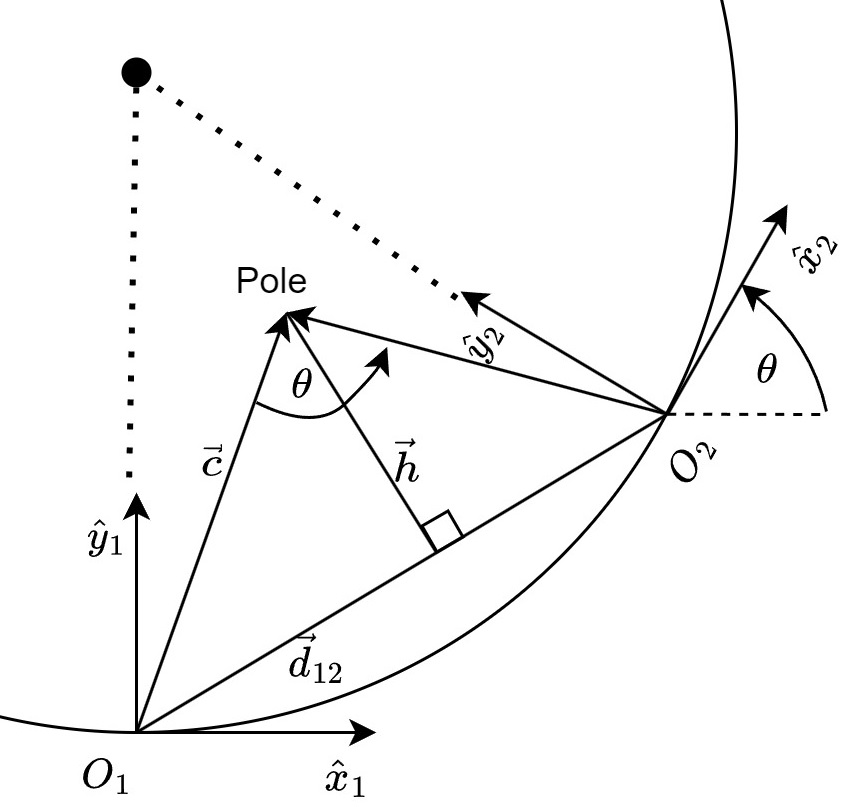
\includegraphics[width=0.25\textwidth]{figures/Poles_roboticsQuartered.jpg}
\end{figure}


\noindent \underline{Quaternions}
\begin{figure}[h!]
    \centering
    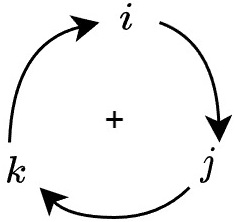
\includegraphics[width=0.10\textwidth]{figures/Quaternions.jpg}
\end{figure}
\begin{equation*}
    \Vec{\Vec{q}} \triangleq a +bi +cj+dk \in \mathds{H} \hspace{30pt} a,\, b,\, c,\, d \in \mathds{R}
\end{equation*}
\begin{equation*}
    \left(\Vec{\Vec{q}}\right)^{-1} = \Vec{\Vec{q}}\,^* / \left\| \Vec{\Vec{q}}\,\right\| \hspace{30pt} i^2=j^2=k^2=ijk=-1
\end{equation*}
\begin{equation*}
    \Vec{\Vec{q}}\Vec{v}\Vec{\Vec{q}} = \cos \left( \frac{\theta}{2}\right) + \sin \left( \frac{\theta}{2}\right) \Vec{v } \hspace{30pt} \Vec{v} \in \mathds{H}\setminus \mathds{R} 
\end{equation*}
\begin{align*}
    \Vec{\Vec{p}}\Vec{\Vec{q}} &= \left(p_0 +\Vec{p} \right) \left(q_0 +\Vec{q} \right) = \text{ (or imaj. number math)}\\
    &=p_0q_0 + p_0\Vec{q} + q_0\Vec{p} + \Vec{p}\times \Vec{q} - \Vec{p}\cdot \Vec{q}
\end{align*}
\end{document}